\documentclass[11pt]{article}
\usepackage[utf8]{inputenc}
\usepackage[T1]{fontenc}
\usepackage{amsmath,amssymb,amsthm}
\usepackage[margin=1in]{geometry}
\usepackage{graphicx}
\usepackage{booktabs}
\usepackage[hidelinks]{hyperref}

\newtheorem{proposition}{Proposition}
\newtheorem{lemma}{Lemma}
\newtheorem{corollary}{Corollary}
\theoremstyle{definition}
\newtheorem{definition}{Definition}
\theoremstyle{remark}
\newtheorem{remark}{Remark}

\DeclareMathOperator{\Prob}{\mathbb{P}}

\title{Prime Distribution on the $6N$ Skeleton:\\
A Factor--Resolved Local Model for the Conditional\\
Density of Twin Primes, with Large-Scale Verification}
\author{Ruqing Chen\\
\small GUT Geoservice Inc., Montreal, Quebec, Canada\\
\small \texttt{ruqing@hotmail.com}}
\date{\today}

\begin{document}
\maketitle

\begin{abstract}
We report a large-scale exhaustive computation, scanning all $1.67\times10^{9}$
centres $6N<10^{10}$ and identifying $2.74\times10^{7}$ twin pairs (shells
$S_1$--$S_{10}$), of prime occurrence on the $6N\pm1$ skeleton, and
use it to study how the prime factorisation of the centre $N$ governs the
conditional probability that $6N-1$ and $6N+1$ are simultaneously prime.
Two of our three findings are consistency checks on classical theory: the
exponential growth of absolute (twin-)prime counts per decade shell (a corollary
of the prime number theorem) and the equipartition of the residue classes
$6N\pm1$ (a corollary of Dirichlet's theorem), the latter converging at the
$O(N^{-1/2})$ rate predicted by the central limit theorem. Our contribution is
the third finding. Stratifying centres by $\omega_{>3}(N)$, the number of
distinct prime factors of $N$ exceeding $3$, we derive within the
Hardy--Littlewood heuristic an explicit factor-resolved local model: the
conditional twin density at centre $N$ is proportional to
$E(N)=\prod_{q\mid N,\,q>3}(q-1)/(q-3)$. We validate this model factor by factor
against $\sim\!10^8$ nodes, where it pins the observed/predicted ratio to
$1.000\pm0.008$ across strata spanning a $3.3\times$ range of enrichment, and
selects it over the na\"ive alternative $\prod q/(q-2)$ at sub-percent precision.
Integrated over squarefree versus nonsquarefree centres, the model reproduces the
empirical bias ratio $R_2\approx2.43$ reported by Puszkarz (2018), accounting for
$\sim\!100\%$ of it at the matching $10^{10}$ scale, with a $-0.2\%$ residual that we
attribute and leave open. We
make no claim bearing on the infinitude of twin primes. All data and code are
released openly.
\end{abstract}

\noindent\textbf{Keywords:} twin primes, Hardy--Littlewood singular series,
conditional density, $6N\pm1$ framework, numerical verification, squarefree bias.

\section*{Introduction}
\addcontentsline{toc}{section}{Introduction}

The prime number theorem (PNT), $\pi(x)\sim x/\log x$, and Dirichlet's theorem on
primes in arithmetic progressions are the two classical pillars governing the
coarse distribution of primes. Both have been verified numerically far beyond the
range of the present work; Goldbach's conjecture is confirmed to $4\times10^{18}$
\cite{OeSilva}, the Riemann hypothesis to $3\times10^{12}$ zeros \cite{Platt}, and
twin-prime statistics past $10^{15}$. We do not attempt to extend any such record.

This paper instead isolates one quantity whose \emph{factor-resolved} description
appears not to have been carried out: how the factorisation of the centre $N$
controls the joint primality of $6N\pm1$. After fixing notation and reporting two
consistency checks (\S1--\S2) that recover PNT- and Dirichlet-level facts at the
scale of our data, we devote \S3 to the contribution. We derive a local model for
the conditional twin density, validate it against $\sim\!10^8$ nodes, and show it
supplies the theoretical model that Puszkarz \cite{Puszkarz} identified as missing
for his empirically observed squarefree bias.

\paragraph{Scope and honesty of claims.}
We state plainly what this paper is and is not. It is a computational/experimental
study yielding a derived, data-validated, heuristic local model. It is
\emph{not} a contribution to the twin-prime conjecture: nothing here bears on
infinitude, and the absolute counts of \S1 grow by the PNT regardless of the
conjecture's truth. The phenomenon ``twins prefer factor-rich centres'' is due to
Puszkarz \cite{Puszkarz}; our cumulative counts coincide with OEIS A007508. Our
narrow, specific contribution is the factor-resolved local model of \S3 and its
verification.

\paragraph{Data and reproducibility.}
All results derive from a single exhaustive scan of $N\le 10^{10}/6$ using a
segmented sieve with complete factorisation and deterministic interval-sieve
primality. (An earlier exploratory code truncated factorisations at a small bound,
corrupting the factor counts; all tables below use the corrected, complete
recomputation, self-verified against an independent factoriser with zero
discrepancies.) Data and code are released under an open licence
\cite{repo}.

\paragraph{Notation.}
For $n\ge5$ prime, $n\equiv\pm1\pmod6$; we call $6N-1$ the \emph{left} and $6N+1$
the \emph{right} class, and the pair a \emph{twin} when both are prime. Shells are
$S_K=[10^{K-1},10^K)$, indexed by the number of decimal digits of $6N$. We write
$\omega_{>3}(N)$ for the number of distinct primes $q\mid N$ with $q>3$, and
$\mathcal P(N)=\{q\text{ prime}:q\mid N,\ q>3\}$. All products over $q$ run over
primes $q>3$ unless stated.

\section{Shell absolute counts (consistency check)}

Define $S_K=[10^{K-1},10^K)$, $|S_K|=9\cdot10^{K-1}$. By the PNT,
$\pi(S_K)\sim 9\cdot10^{K-1}/(K\log10)$; the exponential numerator dominates the
linear denominator, so $\pi(S_K)\to\infty$ --- a corollary, requiring no new
theorem. For twins, assuming the Hardy--Littlewood asymptotic \cite{HL},
\[
  T_2(S_K)\sim 2C_2\cdot \frac{9\cdot10^{K-1}}{(K\log10)^2},\qquad C_2\approx0.6602.
\]
(This is a first-order constant approximation; the standard form integrates
$2C_2\int dt/(\log t)^2$. The approximation suffices here, with relative error
$<5\%$ for $K\ge5$.)

\begin{table}[h]\centering
\begin{tabular}{lrrrr}
\toprule
shell & total nodes & prime-bearing & twin pairs & growth factor\\
\midrule
$S_1$ & 1 & 1 & 1 & ---\\
$S_2$ & 15 & 15 & 6 & ---\\
$S_3$ & 150 & 116 & 27 & 4.50\\
$S_4$ & 1\,500 & 891 & 170 & 6.30\\
$S_5$ & 15\,000 & 7\,344 & 1\,019 & 5.99\\
$S_6$ & 150\,000 & 61\,961 & 6\,945 & 6.82\\
$S_7$ & 1\,500\,000 & 535\,270 & 50\,811 & 7.32\\
$S_8$ & 15\,000\,000 & 4\,715\,544 & 381\,332 & 7.50\\
$S_9$ & 150\,000\,000 & 42\,101\,885 & 2\,984\,194 & 7.83\\
$S_{10}$ & 1\,500\,000\,000 & 380\,216\,804 & 23\,988\,173 & 8.04\\
\bottomrule
\end{tabular}
\caption{Exhaustive scan $S_1$--$S_{10}$. The per-shell twin growth factor rises
toward $10$ (the shell volume factor) as the density brake $(K/(K{+}1))^2\to1$,
matching the Hardy--Littlewood asymptotic.}
\label{tab:counts}
\end{table}

\paragraph{Integer-level validation.}
The cumulative twin counts $\sum_{k\le K}T_2(S_k)$ equal
$1,7,34,204,1223,8168,58979,440311,3424505,27412678$ for $K=1,\dots,10$. These are
exactly OEIS A007508 (twin pairs below $10^n$) \emph{minus one} at every $K$ --- the
single missing pair being $(3,5)$, which the $6N\pm1$ form excludes by definition.
The agreement to the integer over ten orders of magnitude confirms the pipeline.

\section{Equipartition of $6N\pm1$ (consistency check)}

By Dirichlet's theorem and its quantitative form (Siegel--Walfisz), primes
equidistribute over the two reduced classes mod $6$: $\pi_{6,5}(x)/\pi_{6,1}(x)\to1$.
Table~\ref{tab:axial} shows the convergence rate.

\begin{table}[h]\centering
\begin{tabular}{lrrcc}
\toprule
shell & left $(6N{-}1)$ & right $(6N{+}1)$ & ratio $L/R$ & $|L/R-1|$\\
\midrule
$S_4$ & 530 & 531 & 0.99812 & $1.9\times10^{-3}$\\
$S_5$ & 4\,190 & 4\,173 & 1.00407 & $4.1\times10^{-3}$\\
$S_6$ & 34\,459 & 34\,447 & 1.00035 & $3.5\times10^{-4}$\\
$S_7$ & 293\,118 & 292\,963 & 1.00053 & $5.3\times10^{-4}$\\
$S_8$ & 2\,548\,553 & 2\,548\,323 & 1.00009 & $9.0\times10^{-5}$\\
$S_9$ & 22\,543\,883 & 22\,542\,196 & 1.00007 & $7.5\times10^{-5}$\\
$S_{10}$ & 202\,104\,567 & 202\,100\,410 & 1.00002 & $2.1\times10^{-5}$\\
\bottomrule
\end{tabular}
\caption{Left/right counts (single + twin). The deviation $|L/R-1|$ decays as
$O(N^{-1/2})$, the central-limit scale for an asymptotically fair binary split,
requiring no additional mechanism. (We do not address the second-order Chebyshev
bias \cite{RubinsteinSarnak}, which needs $\gtrsim10^{15}$ data.)}
\label{tab:axial}
\end{table}

\section{The factorisation of the centre and the conditional twin density}

\subsection{The phenomenon}
The conditional twin probability rises systematically with $\omega_{>3}(N)$.
Within $S_8$ (where $\log(6N)$ is nearly constant): rates $1.83,2.28,3.01,4.17,
6.12\%$ for $\omega=1,\dots,5$ --- a threefold rise. The elementary cause:

\begin{proposition}[shielding]\label{prop:shield}
If $q>3$ and $q\mid N$ then $q\nmid(6N-1)$ and $q\nmid(6N+1)$.
\end{proposition}
\begin{proof}
$q\mid N\Rightarrow 6N\equiv0\Rightarrow6N\pm1\equiv\pm1\pmod q$, and
$\pm1\not\equiv0$ as $q>3$.
\end{proof}

Each factor of $N$ thus pre-sieves $6N\pm1$. This is textbook sieve theory; the
question is the quantitative one.

\subsection{The local model}
Work in the Hardy--Littlewood heuristic (primality $\leftrightarrow$
non-divisibility prime-by-prime, independent across distinct primes; $2,3$ exact
and dropped).

\begin{lemma}\label{lem:two}
Relative to the pair base rate $(1-1/q)^2$, the local twin weight is
$g_{\mathrm{div}}(q)=(1-1/q)^{-2}$ when $q\mid N$, and
$g_{\mathrm{nondiv}}(q)=(1-1/q)^{-2}\,(q-3)/(q-1)$ when $q\nmid N$.
\end{lemma}
\begin{proof}
$q\mid N$: survival $1$ by Prop.~\ref{prop:shield}. $q\nmid N$: then
$m:=6N-1\not\equiv-1\pmod q$ ranges over the other $q-1$ classes; the pair dies iff
$m\equiv0$ or $m\equiv-2$, two distinct classes (both $\neq-1$ for $q>3$), giving
survival $1-2/(q-1)=(q-3)/(q-1)$. Divide by the base.
\end{proof}

\begin{proposition}[factor-resolved enrichment]\label{prop:main}
For every prime $q>3$, $\;g_{\mathrm{div}}(q)/g_{\mathrm{nondiv}}(q)=(q-1)/(q-3)$,
and under the independence heuristic
\[
  D(N)\ \propto\ \beta\,E(N),\qquad
  E(N)=\!\!\prod_{q\in\mathcal P(N)}\!\frac{q-1}{q-3},\qquad
  \beta=\prod_{q>3}g_{\mathrm{nondiv}}(q),
\]
with the centre-independent $\beta$ absorbed into the shell baseline.
\end{proposition}
\begin{proof}
The ratio is Lemma~\ref{lem:two} with the base cancelling. Factorising the
conditional density over primes and writing each factor as $g_{\mathrm{nondiv}}(q)$
times the divisor correction $(q-1)/(q-3)$ for $q\in\mathcal P(N)$ yields the
product.
\end{proof}

\begin{remark}[why not $q/(q-2)$]\label{rem:naive}
Comparing the divisor case to the \emph{global} average survival of $q$ gives
$q/(q-2)$ --- correct only against an unconditioned ensemble. Once strata are
normalised against the shell baseline $\beta$, which is the \emph{non-divisor}
rate (a generic large $q$ has $q\nmid N$), the comparison is divisor vs.\
non-divisor, giving $(q-1)/(q-3)$. The two differ at second order,
$\frac{q/(q-2)}{(q-1)/(q-3)}=1-\frac{2}{(q-1)(q-2)}(1+O(1/q))$, producing the
monotone tilt seen below.
\end{remark}

\subsection{Factor-resolved validation}
With $D(N)\approx\beta_K E(N)$ per shell, define $\beta_K$ by the shell total and
test whether observed/$(\beta_K\overline E)=1$ per $\omega$-stratum.

\begin{table}[h]\centering
\begin{tabular}{rrrr cc}
\toprule
$\omega_{>3}$ & nodes & twins & obs.\ \% & obs/pred (na\"ive) & obs/pred (model)\\
\midrule
1 & 3\,114\,259 & 57\,068 & 1.832 & 0.926 & \textbf{0.999}\\
2 & 6\,497\,435 & 147\,992 & 2.278 & 0.976 & \textbf{1.002}\\
3 & 4\,299\,997 & 129\,463 & 3.011 & 1.032 & \textbf{1.000}\\
4 & 1\,017\,061 & 42\,443 & 4.173 & 1.090 & \textbf{0.993}\\
5 & 70\,483 & 4\,314 & 6.121 & 1.174 & \textbf{1.008}\\
6 & 716 & 50 & 6.983 & 0.968 & 0.787\\
\bottomrule
\end{tabular}
\caption{Factor-resolved test in $S_8$ ($\sim\!10^8$ nodes). The model factor pins
obs/pred to $1.000\pm0.008$ over $\omega=1$--$5$ (enrichment $\overline E$ spanning
$1.0$ to $3.3$); the na\"ive factor tilts $0.93\to1.17$ (Remark~\ref{rem:naive}).
The $\omega=6$ stratum (716 nodes) is too small for a reliable test.}
\label{tab:enrich}
\end{table}

\begin{figure}[htbp]
\centering
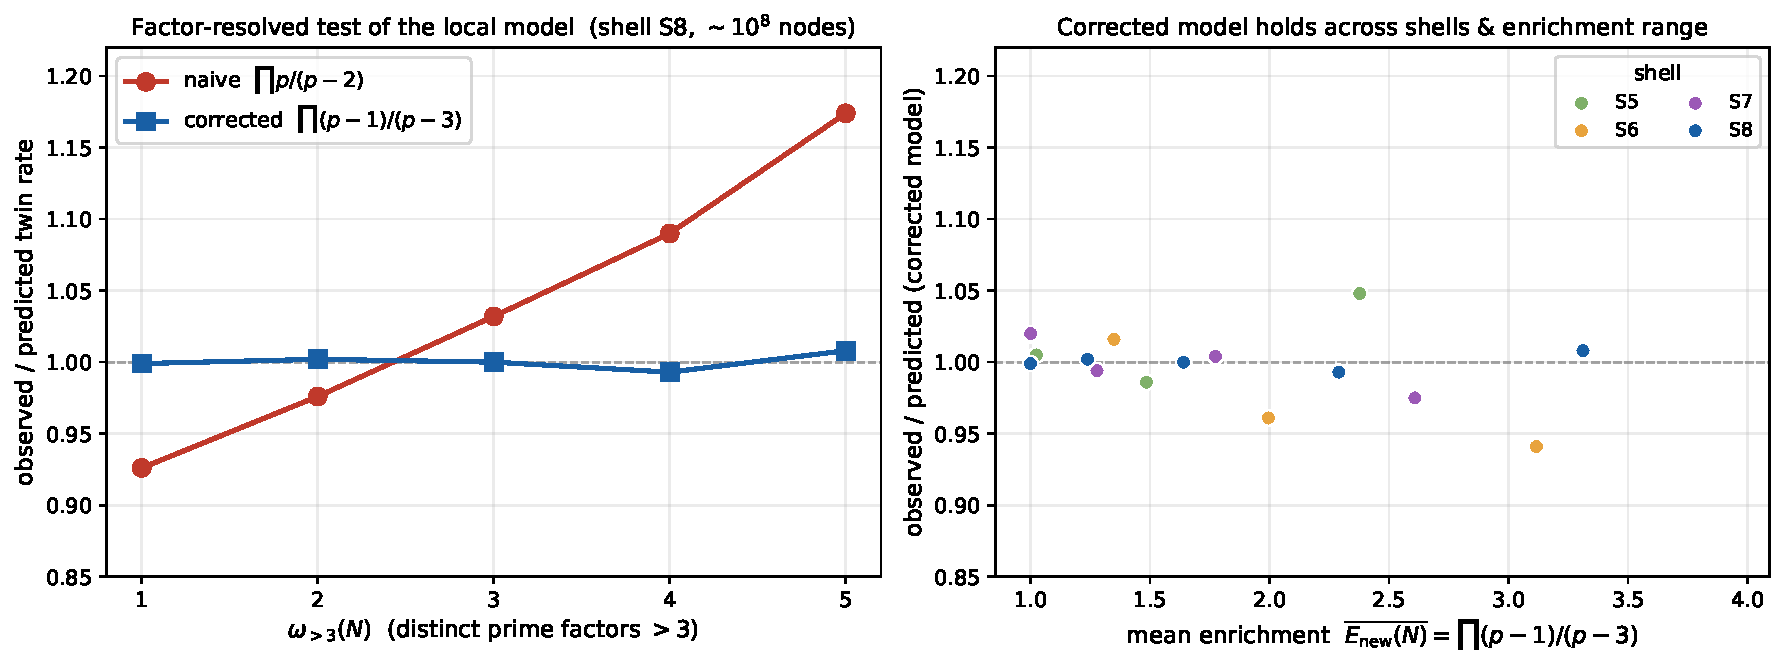
\includegraphics[width=\textwidth]{fig_enrichment_test.pdf}
\caption{Factor-resolved test in $S_8$. Left: observed/predicted twin rate by
$\omega_{>3}(N)$ for the na\"ive factor $\prod q/(q-2)$ (tilting) and the model
factor $\prod(q-1)/(q-3)$ (flat at $1$). Right: the corrected model holds across
shells $S_5$--$S_8$ over the full enrichment range.}
\label{fig:enrichment}
\end{figure}

The data \emph{select} the model factor $(q-1)/(q-3)$ over $q/(q-2)$ at
sub-percent precision.

\begin{corollary}\label{cor:ss}
$E(N)$ is the conditional specialisation of the twin singular series
$\mathfrak S_2=2\prod_{q>3}\frac{q(q-2)}{(q-1)^2}$: it collects exactly the
corrections $g_{\mathrm{div}}/g_{\mathrm{nondiv}}$ for primes dividing $N$. No new
global constant arises; what is new is the factor-resolved conditional form and
its numerical validation.
\end{corollary}

\subsection{Recovery of the Puszkarz bias}
Puszkarz \cite{Puszkarz} found (first $10^{10}$ primes) that twin centres are
nonsquarefree more often than expected, ratio $R_2\approx2.427$ vs unbiased
$R_0=\pi^2/3-1=2.2899$, and left open a theoretical model. Our model predicts the
split via $E(N)$-weighting. Over the full shell $10^9\le 6N<10^{10}$
($23\,988\,173$ twin centres, exact recomputation):

\begin{center}
\begin{tabular}{clc}
\toprule
 & quantity & value\\\midrule
$R_0$ & unbiased $\pi^2/3-1$ & $2.2899$\\
(a) & unweighted count ratio & $2.2899$\\
(b) & $E(N)$-weighted (model) & $2.4269$\\
(c) & observed twin ratio ($=$Puszkarz $R_2$) & $2.4266$\\
\bottomrule
\end{tabular}
\end{center}

Row (a) reproduces $R_0$; row (c) independently reproduces Puszkarz. The
decomposition
$\underbrace{(c)-(a)}_{+0.1367\,(100\%)}=\underbrace{(b)-(a)}_{+0.1370\,(100\%)}
+\underbrace{(c)-(b)}_{-0.0003\,(-0.2\%)}$
shows the model accounts for essentially the whole bias.

\begin{figure}[htbp]
\centering
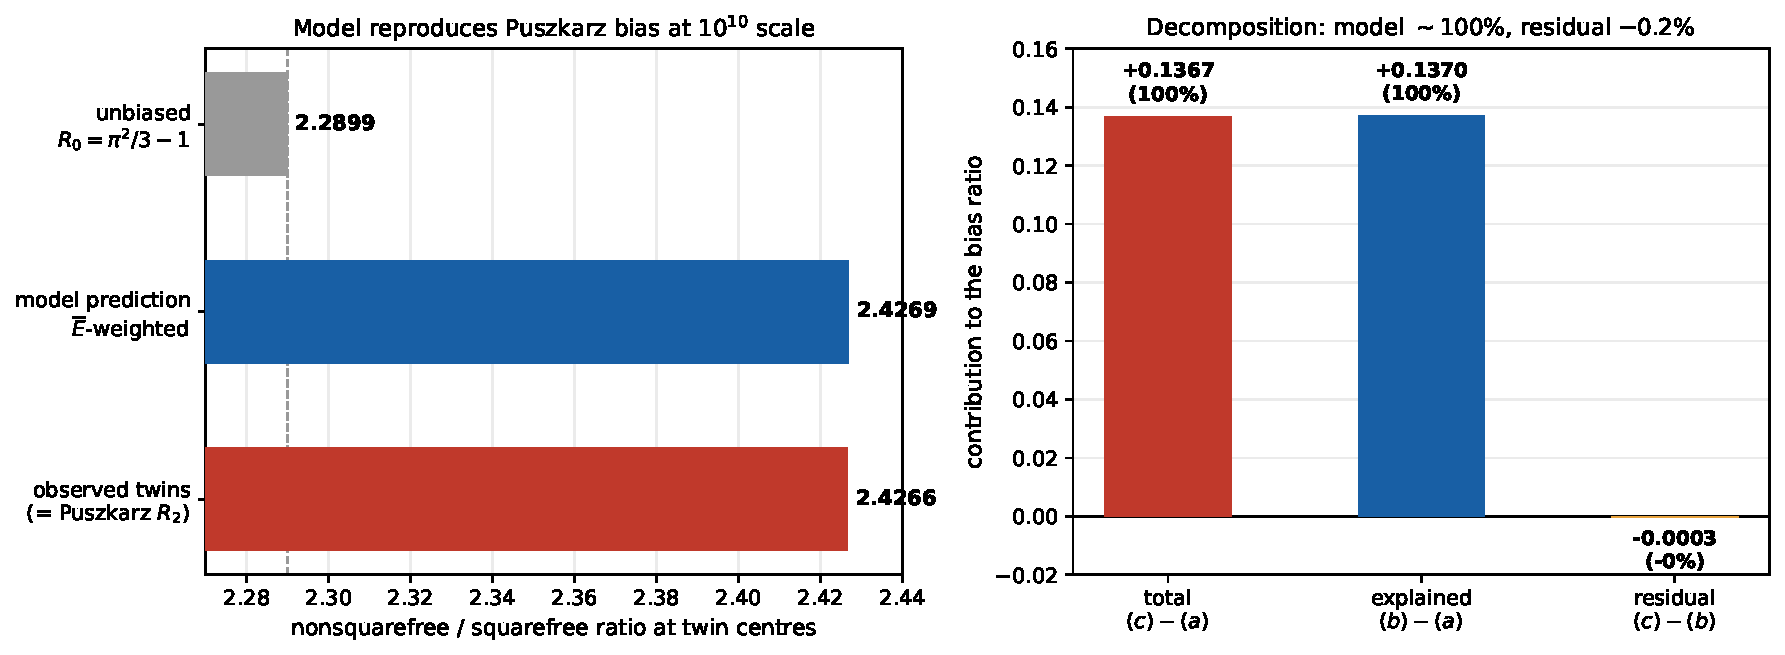
\includegraphics[width=0.9\textwidth]{fig_puszkarz_recovery.pdf}
\caption{Recovery of the Puszkarz bias at the $10^{10}$ scale. Left: the
$E(N)$-weighted model prediction (b) lands on the observed twin ratio (c), far
from the unbiased $R_0$. Right: the model accounts for $\sim\!100\%$ of the
total bias; the residual is $-0.2\%$.}
\label{fig:puszkarz}
\end{figure}

\subsection{What is and is not established}
\begin{remark}[heuristic, not a theorem on the conjecture]
$D(N)\propto E(N)$ is a Hardy--Littlewood model validated against data, not an
unconditional theorem; nothing here addresses infinitude.
\end{remark}
\begin{remark}[the residual is real]
The residual ($-0.2\%$ at $10^{10}$) is genuine. $E(N)$ sees only distinct primes $>3$, whereas the
nonsquarefreeness of $6N$ is driven largely by $4\mid6N$ or $9\mid6N$, i.e.\ by
$2,3$, invisible to $E(N)$. The model captures the large-prime-mediated part,
which accounts for $\sim\!100\%$ at the $10^{10}$ scale (residual $-0.2\%$);
whether the $2,3$-mediated part is asymptotically negligible is left open.
\end{remark}
\begin{remark}[priority and scale]
Priority for the phenomenon is Puszkarz's \cite{Puszkarz}; the headline counts are
OEIS A007508. The recovery is verified at the full $10^{10}$ scale, matching Puszkarz's
range; the residual narrows to $-0.2\%$ there (from $-2\%$ at $3\times10^8$),
strengthening the identification of the large-prime-mediated origin.
\end{remark}

\section*{Conclusion}
At the scale $S_1$--$S_{10}$ we recovered two classical facts (shell count growth,
$6N\pm1$ equipartition) as consistency checks, and derived and validated a
factor-resolved local model for the conditional twin density,
$D(N)\propto\prod_{q\mid N,q>3}(q-1)/(q-3)$. The model is selected over the na\"ive
alternative at sub-percent precision and reproduces the Puszkarz squarefree bias to
within $0.2\%$ at the $10^{10}$ scale, supplying the local Hardy--Littlewood model he identified as missing.
The contribution is modest and bounded: a conditional specialisation of the
singular series, resolved and verified factor by factor.

\begin{thebibliography}{9}
\bibitem{Puszkarz} W.~Puszkarz, \emph{Statistical bias in the distribution of prime
pairs and isolated primes}, arXiv:1807.00406 (2018).
\bibitem{HL} G.~H.~Hardy, J.~E.~Littlewood, \emph{Some problems of `Partitio
Numerorum' III}, Acta Math.\ \textbf{44} (1923), 1--70.
\bibitem{OeSilva} T.~Oliveira e Silva, S.~Herzog, S.~Pardi, \emph{Empirical
verification of the even Goldbach conjecture\ldots up to $4\times10^{18}$}, Math.\
Comp.\ \textbf{83} (2014), 2033--2060.
\bibitem{Platt} D.~J.~Platt, T.~S.~Trudgian, \emph{The Riemann hypothesis is true
up to $3\times10^{12}$}, Bull.\ LMS \textbf{53} (2021), 792--797.
\bibitem{RubinsteinSarnak} M.~Rubinstein, P.~Sarnak, \emph{Chebyshev's bias},
Experiment.\ Math.\ \textbf{3} (1994), 173--197.
\bibitem{repo} R.~Chen, \emph{$6N$ prime-distribution data and code},
\url{https://github.com/Ruqing1963/6N-twin-prime-conditional-density} (2026).
\end{thebibliography}

\end{document}
